\documentclass[a4paper]{article}
\usepackage{ctex}
\usepackage[affil-it]{authblk}
\usepackage{float}
\usepackage{amsmath, amssymb, amsthm, amsfonts}
% \usepackage[backend=bibtex,style=numeric]{biblatex}
\usepackage{graphicx}

\usepackage{hyperref}
% 设置超链接样式
\hypersetup{
	colorlinks=true,
	linkcolor=blue,
	citecolor=blue,
	urlcolor=blue,
}

\usepackage{geometry}
\geometry{margin=1.5cm, vmargin={0pt,1cm}}
\setlength{\topmargin}{-1cm}
\setlength{\paperheight}{29.7cm}
\setlength{\textheight}{25.3cm}

% \addbibresource{citation.bib}

\begin{document}
% =================================================
\title{Numerical Analysis homework \# 2}

\author{王昊 Wang Hao 3220104819
  \thanks{Electronic address: \texttt{3220104819@zju.edu.cn}}}
\affil{(Mathematics and Applied Mathematics 2201), Zhejiang University }


\date{Due time: \today}

\maketitle

% \begin{abstract}
%     The abstract is not necessary for the theoretical homework, 
%     but for the programming project, 
%     you are encouraged to write one.      
% \end{abstract}


% ============================================
\section*{I. Error and Its Bounds About Interpolation}

\subsection*{I-a Find $\xi(x)$}

For $f(x) = \frac{1}{x}, x_0=1, x_1=2$, we can easily get the Interpolation polynomial $p_1(f; x)$ as follows:
\begin{equation}
  p_1(f; x) = f(x_0) \frac{x-x_1}{x_0-x_1} + f(x_1) \frac{x-x_0}{x_1-x_0} = -\frac{1}{2} x + \frac{3}{2} .
\end{equation}
So by $f(x) - p_1(f; x) = \frac{f^{\prime \prime} (\xi (x))}{2} (x-x_0) (x-x_1)$, we can get $\xi(x)$ as follows:
\begin{equation}
  \begin{aligned}
    f^{\prime \prime} (\xi (x)) &= \frac{1}{x}, \\
    \Rightarrow \xi (x) = &\sqrt[3]{2x}.
  \end{aligned}
\end{equation}
\subsection*{I-b Find the Bounds of $\xi(x)$}

We already know that $\xi(x) = \sqrt[3]{2x}$, so in the domain $[1,2]$, we can easily know that:
\begin{equation}
  \min \xi(x) = \sqrt[3]{2}, \quad \max \xi(x) = \sqrt[3]{4},
\end{equation}
and $f^{\prime \prime}(\xi(x)) = \frac{1}{x}$. Therefore we can know
\begin{equation}
  \max f^{\prime \prime}(\xi(x)) = \frac{1}{1} = 1. 
\end{equation}

\section*{II. Interpolation on $\mathbb{P}_{m}^+$}

In order to find $p \in \mathbb{P}_{2n}^+ = \{p: p\in \mathbb{P}_{2n}, \forall x\in\mathbb{R}, p(x)\ge 0\}$, we need to find new basis functions $\{l_i(x)\}_{i=0}^{n}$, which $l_i \in \mathbb{P}_{2x}^+$. 

It is easy to know that the following functions is enough:
\begin{equation}
  l_i(x) = \prod_{k=0, k\neq i}^{n} \cfrac{(x-x_k)^2}{(x_i-x_k)^2}, \quad i=0,1,\cdots,n.
\end{equation}
which satifies $l_i(x_i) = 1, l_i(x_j) = 0, j\neq i, l_i(x) \ge 0, \forall x\in\mathbb{R}$.

So the polynomial $p \in \mathbb{P}_{2n}^+$ such that $p(x_i) = f(x_i) \ge 0, i=0,1,\cdots,n$ can be written as
\begin{equation}
  p(x) = \sum_{i=0}^{n} f(x_i) l_i(x) = \sum_{i=0}^{n} f(x_i) \prod_{k=0, k\neq i}^{n} \cfrac{(x-x_k)^2}{(x_i-x_k)^2}.
\end{equation}
\section*{III. Evaluation for Exponential Function}

\subsection*{III-a. Calculate $f[t,t+1,\cdots, t+n]$}

In order to prove when $f(x) = e^t$ then $\forall t\in \mathbb{R}, f[t,t+1,\cdots, t+n] = \frac{(e-1)^n}{n!}e^t$.

\begin{itemize}
  \item When $n=0$, we can easily know that $f[t] = e^t = \frac{(e-1)^0}{0!}e^t$. 
  \item Assume then when $n=k$, the equation holds, i.e. $f[t,t+1,\cdots, t+k] = \frac{(e-1)^k}{k!}e^t$. 
  Then, for $n=k+1$, we can easily know
  \begin{equation}
    \begin{aligned}
      f[t,t+1,\cdots, t+k+1] &= \frac{f[t+1,\cdots, t+k+1] - f[t,t+1,\cdots, t+k]}{(t+k+1) - t} \\
                             &= \frac{\frac{(e-1)^k}{k!} (e^{t+1} - e^t)}{k+1} \\
                             &= \frac{(e-1)^{k+1}}{(k+1)!}e^t. 
    \end{aligned}
    \label{eq::III-a.1}
  \end{equation}

  The equation holds for $n=k+1$.
\end{itemize}

Therefore, we can know that $\forall t\in \mathbb{R}, f[t,t+1,\cdots, t+n] = \frac{(e-1)^n}{n!}e^t$. 

\subsection*{III-b. Error Estimation}

From the equation \ref{eq::III-a.1}, we can know that
\begin{equation}
    f[t,t+1,\cdots, t+n] = \frac{(e-1)^n}{n!}e^t, \forall t\in \mathbb{R}. 
\end{equation}

Therefore, we can easily know
\begin{equation}
  \begin{aligned}
    f[0,1,\cdots, n] &= \frac{(e-1)^n}{n!} = \frac{f^{(n)}(\xi)}{n!} = \frac{e^{\xi}}{n!}, \\
    \Rightarrow \xi &= n \ln(e-1) \approx 0.5413n.
  \end{aligned}
\end{equation}

Therefore, $\xi = n \ln(e-1)$, and $\xi$ is to the right of the midpoint $\frac{n}{2}$.

\section*{IV. Application of Newton Interpolation}

\subsection*{IV-a. Find the Newton Interpolation Polynomial}

For $f(0)=5, f(1)=3, f(3)=5, f(4)=12$, we can know that $f[0]=5, f[1]=3, f[3]=5, f[4]=12$. Draw table like this:

\begin{table}[H]
  \centering
  \begin{tabular}{c|cccc}
    0 & 5  &    &   &\\
    1 & 3  & -2 &   &\\
    3 & 5  & 1  & 1 &\\
    4 & 12 & 7  & 2 & $\frac{1}{4}$\\
  \end{tabular}
  \label{tabel::IV-A.tabel1}
\end{table}

The above table \ref{tabel::IV-A.tabel1} is given by $f[x_0,x_1,\cdots,x_n] = \frac{f[x_1,\cdots,x_n] - f[x_0,x_1,\cdots,x_{n-1}]}{x_n - x_0}$, so we can know that $f[0]=5, f[0,1]=-2, f[0,1,3]=1, f[0,1,3,4]=\frac{1}{4}$. 

Therefore the Newton Interpolation is
\begin{equation}
  \begin{aligned}
    p_3(f;x) &= f[0] + f[0,1](x-0) + f[0,1,3](x-0)(x-1) + f[0,1,3,4](x-0)(x-1)(x-3) \\
             &= 5 - 2x + x(x-1) + \frac{1}{4}x(x-1)(x-3) \\
             &= \frac{1}{4}x^3 - \frac{9}{4}x + 5.
  \end{aligned}
\end{equation}

\section*{IV-b. Minimum value of $p_3(f;x)$}

In order to find the approximate minimum value of $f(x)$ in $x\in (1,3)$, we can just analyze the minimum value of $p_3(f;x) = p(x)$ in $x\in(1,3)$.

It iss easy to show $p(x) = \frac{1}{4}x^3 - \frac{9}{4}x + 5$, so we can know that 
\begin{equation}
  p^{\prime}(x) = \frac{3}{4}x^2 - \frac{9}{4} = 0 \Rightarrow x = \sqrt{3}.
\end{equation}

Therefore, the minimum value of $p(x)$ in $x\in(1,3)$ is $p(\sqrt{3}) = 5 - \frac{3}{2}\sqrt{3}$, $x_{\min} = \sqrt{3}$.

\section*{V. The Generalized Newton Interpolation}

\subsection*{V-a. Compute the Generalized Newton Interpolation}

To compute $f[0,1,1,1,2,2]$, we can draw the table like this:

\begin{table}[H]
  \centering
  \begin{tabular}{c|cccccc}
    0 & $f[0]$ &                 &                                  & & & \\
    1 & $f[1]$ & $f[0,1]$        &                                  & & & \\
    1 & $f[1]$ & $f^{\prime}(1)$ & $f[0,1,1]$                       & & & \\
    1 & $f[1]$ & $f^{\prime}(1)$ & $\frac{f^{\prime \prime}(1)}{2}$ & $f[0,1,1,1]$ & & \\
    2 & $f[2]$ & $f[1,2]$        & $f[1,1,2]$                       & $f[1,1,1,2]$ & $f[0,1,1,1,2]$ & \\
    2 & $f[2]$ & $f^{\prime}(2)$ & $f[1,2,2]$                       & $f[1,1,2,2]$ & $f[1,1,1,2,2]$ & $f[0,1,1,1,2,2]$ \\
  \end{tabular}
  \label{tabel::V-A.tabel1}
\end{table}

We can know that $f(x) = x^7, f^\prime(x)=7x^6, f^{\prime \prime}(x) = 42x^5$, so put them into the table \ref{tabel::V-A.tabel1}, we can get:

\begin{table}[H]
  \centering
  \begin{tabular}{c|cccccc}
    0 & 0   &     &     &     &     & \\
    1 & 1   & 1   &     &     &     & \\
    1 & 1   & 7   & 6   &     &     & \\
    1 & 1   & 7   & 21  & 15  &     & \\
    2 & 128 & 127 & 120 & 99  & 42  & \\
    2 & 128 & 448 & 321 & 201 & 102 & 30 \\
  \end{tabular}
  \label{tabel::V-A.tabel2}
\end{table}

So $f[0,1,1,1,2,2] = 30$.

\subsection*{V-b. Determin $\xi$}
We know that $f[0,1,1,1,2,2] = \frac{f^{(5)}(\xi)}{5!}$, and $f^{(5)}(x) = 2520x^2$, so we can know that:

\begin{equation}
  \begin{aligned}
    30 &= f[0,1,1,1,2,2] = \frac{f^{(5)}(\xi)}{5!} = \frac{2520\xi^2}{5!}, \\
    \Rightarrow \xi &= \sqrt{\frac{5! \times 30}{2520}} = \sqrt{\frac{10}{7}} \approx 1.1952.
  \end{aligned}
\end{equation}

\section*{VI. Hermite Interpolation}
\subsection*{VI-a. Find the Hermite Interpolation Polynomial}
For $f(0)=1,f(1)=2,f^{\prime}=-1,f(3)=f^{\prime}(3)=0$, we can get the following table:

\begin{table}[H]
  \centering
  \begin{tabular}{c|ccccc}
    0 & 1 &     &     &     & \\
    1 & 2 & 1   &     &     & \\
    1 & 2 & -1  & -2   &     & \\
    3 & 0 & -1  & 0  & $\frac{2}{3}$  & \\
    3 & 0 & 0   & $\frac{1}{2}$ & $\frac{1}{4}$  &$-\frac{5}{36}$ \\
  \end{tabular}
  \label{tabel::VI-A.tabel1}
\end{table}

So the Hermite Interpolation Polynomial is
\begin{equation}
  p(x) = 1 + x - 2x(x-1) + \frac{2}{3}x(x-1)^2 - \frac{5}{36}x(x-1)^2(x-3),
\end{equation}
and $p(2) = 0.611111$. 

\subsection*{VI-b. Find the error bound}
From the textbook, we know that the reminder $R(x)$ can be written as follows:
\begin{equation}
  \forall x \in [0,3], R(x) = \frac{f^{(5)} (\xi)}{5!} x(x-1)^2(x-3)^2, \quad \xi \in (0,3).
\end{equation}

Therefore, for $g(x) = x(x-1)^2(x-3)^2$, we have $g^{\prime}(x)=(x-1)(x-3)(5x^2-12x+3) = 0 \Rightarrow x=1,3,\frac{6\pm \sqrt{21}}{5}$. So $\max_{x\in[0,3]} g(x) = g(\frac{6+\sqrt{21}}{5}) \approx 2.05944$. 

In conclusion, we can know that:
\begin{equation}
  \vert R(x)\vert \leq 0.017162 M, \forall x \in [0,3].
\end{equation}

For above answer, we only need to set $x=2$, and then we get
\begin{equation}
  \vert R(2) \vert \leq \frac{M}{60}.
\end{equation}

\section*{VII. Difference Proof}
To prove that for $x_j = x+jh$, we have:
\begin{equation}
  \begin{aligned}
    \Delta^k f(x) &= k! h^k f[x_0, x_1, \cdots, x_k],\\
    \nabla^k f(x) &= k! h^{k} f[x_0, x_{-1}, \cdots, x_{-k}].
  \end{aligned}
  \label{eq::VII.1}
\end{equation}
We prove by induction, $x_j = x+jh$.

(1) For $k=1$, $\Delta f(x) = f(x+h) - f(x) = h f[x_0, x_1],\quad \nabla f(x) = f(x) - f(x-h) = h f[x_0, x_{-1}]$. So\eqref{eq::VII.1} is true.

(2) Assume that for $k$ we have 
\begin{equation}
  \begin{aligned}
    \Delta^k f(x) &= k! h^k f[x_0, x_1, \cdots, x_k],\\
    \nabla^k f(x) &= k! h^{k} f[x_0, x_{-1}, \cdots, x_{-k}].
  \end{aligned}
\end{equation}

Then for $k+1$, we have the following:
\begin{equation}
  \begin{aligned}
    \Delta^{k+1} f(x) &= \Delta^k f(x+h) - \Delta^k f(x) = \Delta^k f(x_1) - \Delta^k f(x_0) \\
    &= k! h^k f[x_1, x_2, \cdots, x_{k+1}] - k! h^k f[x_0, x_1, \cdots, x_k] \\
    &= k! h^k (x_{k+1} - x_0) \frac{f[x_1, x_2, \cdots, x_{k+1}] - k! h^k f[x_0, x_1, \cdots, x_k]}{x_{k+1} - x_0} \\
    &= (k+1)! h^{k+1} f[x_0, x_1, \cdots, x_{k+1}].
  \end{aligned}
\end{equation}

\begin{equation}
  \begin{aligned}
    \nabla^{k+1} f(x) &= \nabla^k f(x) - \nabla^k f(x-h) = \nabla^k f(x_0) - \nabla^k f(x_{-1}) \\
    &= k! h^{k} f[x_0, x_{-1}, \cdots, x_{-k}] - k! h^{k} f[x_{-1}, x_{-2}, \cdots, x_{-k-1}] \\
    &= k! h^{k} (x_0 - x_{-k-1}) \frac{f[x_0, x_{-1}, \cdots, x_{-k}] - f[x_{-1}, x_{-2}, \cdots, x_{-k-1}]}{x_0 - x_{-k-1}} \\
    &= (k+1)! h^{k+1} f[x_0, x_{-1}, \cdots, x_{-k-1}].
  \end{aligned}
\end{equation}

Therefore, the relation\eqref{eq::VII.1} is true for $\forall k \in \mathbb{N}$.

\section*{VIII. Differential of Difference}
When $f$ is differentiable at $x_0$, then 
\begin{equation}
  \frac{\partial f[x_0, x_1, \cdots, x_k]}{\partial x_0} = \lim_{x_t \rightarrow x_0}\frac{f[x_0, x_1, \cdots, x_k] - f[x_t, x_1, \cdots, x_k]}{x_0 - x_t} = \lim_{x_t\rightarrow x_0} f[x_0, x_t, x_1, \cdots, x_k].
\end{equation}

We can know that $\lim_{x_t \rightarrow x_0} f(x_t) = f(x_0), \lim_{x_t \rightarrow x_0} f^{\prime}(x_t) = f^{\prime} (x_0)$. From the difference table 

\begin{table}[H]
  \centering
  \begin{tabular}{c|cccccc}
    $x_0$ & $f[x_0]$ &                 &                                  & & & \\
    $x_t$ & $f[x_t]$ & $f[x_0,x_t]$        &                                  & & & \\
    $x_1$ & $f[x_1]$ & $f[x_1,x_t]$& $\cdots $                      & & & \\
    $\cdots$ \\ 
    $x_k$ & $f[x_k]$ & $f[x_{k-1}, x_k]$ & $\cdots$ & $f[x_0,x_t,\cdots,x_k]$\\
  \end{tabular}
  \label{tabel::VIII.tabel1}
\end{table}
we can know that $f[x_0,x_t,\cdots,x_k]$ is a linear combination of $f[x_0,x_t]\cdots f[x_{k-1},x_k]$, and the coefficient is given by $x_0\cdots x_k$. We know that the four basic arithmetic operations on continuous functions still result in continuous functions. Therefore, $f[x_0,x_t,\cdots,x_k]$ is continuous at $x_t$, $\lim_{x_t \rightarrow x_0} f[x_0,x_t,\cdots,x_k] = f[x_0,x_0,\cdots,x_k]$. So we have
\begin{equation}
  \frac{\partial f[x_0, x_1, \cdots, x_k]}{\partial x_0} = \lim_{x_t\rightarrow x_0} f[x_0, x_t, x_1, \cdots, x_k] = f[x_0,x_0,x_1,\cdots, x_k].
\end{equation}


\section*{IX. Min-Max Problem}
For $f(x) = a_0x^n + a_1x^{n-1} + \cdots + a_n, \forall x\in[a,b]$, we can let $x = \frac{b-a}{2} t + \frac{b+a}{2}, \forall t\in[-1,1]$. Thus we have $f(x) = a_0(\frac{b-a}{2} t + \frac{b+a}{2})^n + \cdots + a_n = b_0 t^n+ b_1 t^{n-1} + \cdots + b_n = g(t)$. 

Because $a_0$ is fixed, $b_0 = a_0 (\frac{b-a}{2})^n$, and $a_1, \cdots a_n$ are arbitrary. Consequently $b_1, \cdots, b_n$ are arbitrary. Therefore, the min-max problem of $f(x)$ is equivalent to the min-max problem of $g(t)$.

Define $T_n(t) = \frac{b_0}{2^{n-1}} \cos(n\arccos(t))$. Next we will prove
\begin{equation}
  \frac{b_0}{2^{n-1}} = \max_{t\in[-1,1]} \vert T_n(t) \vert \le \max_{t\in[-1,1]} \vert g(t) \vert.
\end{equation}

We will use a proof by contradiction. Assume that $\max_{t\in[-1,1]} \vert g(t) \vert < \frac{b_0}{2^{n-1}}$. And let $x_0, \cdots, x_n$ denote the zero of $T^{\prime}_n(t)$ in $[-1,1]$.

Let $Q(t) = T_n(t) - g(t)$, we have
\begin{equation}
  Q(x_k) = (-1)^k \frac{b_0}{2^{n-1}} - g(x_k), \quad k=0,\cdots n.
\end{equation}
Because $\max_{t\in[-1,1]} \vert g(t) \vert < \frac{b_0}{2^{n-1}}$, so $Q(x)$ have $n$ roots in $[-1,1]$. But $Q(t)$ is a polynomial of order $n-1$, at most have $n-1$ roots, which is a contradiction. 

Therefore we have
\begin{equation}
  \min_{a_1,\cdots,a_n\in\mathbb{R}} \max_{x\in[a,b]} \vert f(x) \vert = \min_{b_1,\cdots,b_n \in \mathbb{R}} \max_{t\in[-1,1]} \vert g(t) \vert = \frac{b_0}{2^{n-1}} = \frac{1}{2^{n-1}} a_0 (\frac{b-a}{2})^n 
\end{equation}


\section*{X. Imitate the proof of Chebyshev Theorem}
We have $\hat{p}(x) = \frac{T_n(x)}{T_n(a)}$, $p(x) \in \mathbb{P}^a_n$, so we have $\hat{p}(a) = p(a) = 1$. 

Assume that $\Vert p(x) \Vert _{\infty} < \Vert \hat{p}(x) \Vert$. Let $x_0,\cdots,x_n$ denote the zeros of $\hat{p}^{\prime}(x)$ in $[-1,1]$, and define $Q(x) = \hat{p}(x) - p(x)$. We have
\begin{equation}
  Q(x_k) = (-1)^k \frac{2^{n-1}}{T_n(a)} - p(x_k), \quad k=0,\cdots n.
\end{equation}
Therefore, $n$ roots in $[-1,1]$, plus the root $a > 1$. So the polynomial $Q(x)$ of order $n$ has $n+1$ roots, which means it's a constant, which gives a contradiction. 

Therefore 
\begin{equation}
  \forall p \in \mathbb{P}^a_n, \quad \Vert \hat{p}(x) \Vert_{\infty} \leq \Vert p(x) \Vert _{\infty}.
\end{equation}

\section*{XI. Proof of Lemma2.53}
In this section, we will prove 
\begin{equation}
  b_{n-1,k}(t) = \frac{n-k}{n} b_{n,k}(t) + \frac{k+1}{n} b_{n,k+1}(t). 
\end{equation}

By definition, we have
\begin{equation}
  \begin{aligned}
    b_{n-1,k}(t) &= C_{n-1}^k t^k (1-t)^{n-1-k}, \\
    b_{n,k}(t) &= C_n^k t^k (1-t)^{n-k}, \\
    b_{n,k+1}(t) &= C_n^{k+1} t^{k+1} (1-t)^{n-k-1}.
  \end{aligned}
\end{equation}

Therefore, we can know that
\begin{equation}
  \begin{aligned}
    \frac{n-k}{n} b_{n,k}(t) + \frac{k+1}{n} b_{n,k+1}(t) &= \frac{n-k}{n} C_n^k t^k (1-t)^{n-k} + \frac{k+1}{n} C_n^{k+1} t^{k+1} (1-t)^{n-k-1} \\
    &= t^k (1-t)^{n-k-1} \left(\frac{n-k}{n}C_n^k(1-t) + \frac{k+1}{n}C_n^{k+1}t \right) \\
    &= t^k (1-t)^{n-k-1} \left(C_{n-1}^k + (\frac{k+1}{n}C_n^{k+1} - \frac{n-k}{n}C_n^k)t\right) \\
    &= t^k (1-t)^{n-k-1} \left(C_{n-1}^k + (\frac{k+1}{n} \frac{n!}{(n-k-1)!(k+1)!} - \frac{n-k}{n} \frac{n!}{(n-k)!k!})t\right) \\
    &= C_{n-1}^k t^k (1-t)^{n-1-k} = b_{n-1,k}(t),
  \end{aligned}
\end{equation}
which finishes the proof.


\section*{XII. Proof of Lemma2.55}
In this section, we will prove
\begin{equation}
  \forall k=0,1,\cdots,n,\quad \int_{0}^{1} b_{n,k}(t) dt = \frac{1}{n+1}.
\end{equation}

By definition, we have $b_{n,k}(t) = C_n^k t^k (1-t)^{n-k}$. We denote $\int_{0}^{1} b_{n,k}(t) dt$ as $I_{n,k}$. Therefore, for $k=n$, we have
\begin{equation}
  I_{n,n} = \int_{0}^{1} b_{n,n}(t) dt = \int_{0}^{1} C_n^n t^n dt = \frac{1}{n+1}.
\end{equation}

For $k \in \mathbb{N}$ and $k < n$, we have
\begin{equation}
  \begin{aligned}
    I_{n,k} = \int_{0}^{1} b_{n,k}(t) dt &= C_n^k \int_{0}^{1} t^k (1-t)^{n-k} dt \\
    &= \frac{C_n^k}{k+1} \int_{0}^{1} (1-t)^{n-k} d t^{k+1} \\
    &= \frac{C_n^k}{k+1} \left[t^{k+1}(1-t)^{n-k} \vert_0^1 + (n-k)\int_{0}^{1}t^{k+1}(1-t)^{n-k-1} dt \right] \\
    &= \frac{C_n^k}{k+1} (n-k) \int_{0}^{1}t^{k+1}(1-t)^{n-k-1} dt \quad (k\ne n, ~~t^{k+1}(1-t)^{n-k} \vert_0^1 = 0) \\
    &= C_n^{k+1} \int_{0}^{1}t^{k+1}(1-t)^{n-k-1} \\
    &= I_{n,k+1}.
  \end{aligned}
\end{equation}

Therefore, we can know that $\forall k=0,1,\cdots,n,~I_{n,k} = I_{n,k+1} = \cdots = I_{n,n} = \frac{1}{n+1}$, which finishes the proof. 

% ===============================================
% \section*{ \center{\normalsize {Acknowledgement}} }
% The section title is generated by \textbf{Kimi}, with a little revise. 
% \begin{figure}[H]
%   \begin{center}
%     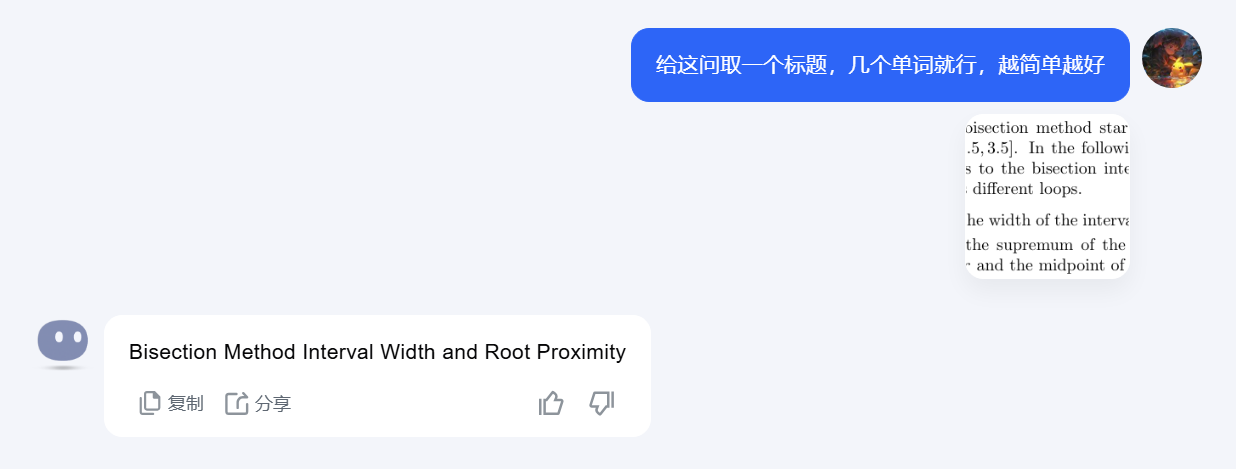
\includegraphics[width=0.8\textwidth]{./figure/kimi.png}
%   \end{center}
% \end{figure}

% \printbibliography


\end{document}